\section{Code}
\subsection{Programmiersprache}

\subsection{Bibliotheken}

\section{Funktionsweise}
Um die zeitlichen Abstand von zwei Fahrzeugen auf einer Route zu ermitteln, sind vorab mehrere Schritte notwendig. Grundlage der Berechnung sind die GPS Koordinaten der Fahrzeuge und der Routenverlauf. Zudem werden sogenannte Messfahrten auf der Route ben�tigt, um die zeitliche Entfernung n�herungsweise zu bestimmten.
 
Als erstes m�ssen alle Fahrzeuge, die auf der gleichen Route fahren aus der Datenbank ermittelt werden. Bei den GPS Daten zu den einzelnen Fahrzeugen handelt es sich um bereits bearbeitete GPS Koordinaten. Die Koordinaten werden vorab im PUT Request (\ref{sub:vehicle:put}) bearbeitet, das hei�t die ungenaue Position des Handy wird auf dichtesten Punkt der Route verschoben. Mit diesen Koordinaten wird anschlie�end f�r jedes Fahrzeug die Entfernung zum Startpunkt der Route berechnet.

F�r die Berechnung der Entfernung zwischen zwei Koordinaten auf der Route (LineString), wird jeweils die Abstand zwischen zwei Punkten des LineStrings ermittelt und aufsummiert. F�r diese Berechnung wird die Haversine Formel verwendet. % TODO Quelle + Recherche https://www.htmlgoodies.com/beyond/javascript/calculate-the-distance-between-two-points-in-your-web-apps.html
 Dieses Verfahren ist n�tig, da die zwei Punkte mit der Route im seltensten Fall eine Gerade bilden (siehe Abbildung \ref{img:route}). Als n�chstes wird der Abstand zwischen den Fahrzeugen in Metern bestimmt. F�r diese Berechnung wird ein Fahrzeug ausgew�hlt (siehe \ref{sub:vehicle:list}), woraufhin die Entfernungen zu den anderen Fahrzeugen ermittelt wird.
 
 Der letzte Schritt ist die Berechnung des zeitlichen Abstandes. Hierf�r sind die Messfahren notwendig. Bei einer Messfahrt wurde im Vorfeld die komplette Route abgefahren und zu regelm��igen Zeitpunkten die GSP Position gemessen. Diese Position wird mit Uhrzeit zusammen in der Datenbank persistiert. Somit ist es m�glich zu bestimmen, wie lange ein Fahrzeug von Position A zu Position B braucht. Im besten Fall existieren mehrere Messfahrten zu einer Route, damit die Aussage genauer wird.
Um nun die zeitliche Entfernung von Fahrzeug A zu Fahrzeug B zu ermitteln, wird der dichteste Punkt von einer Messfahrt zum Fahrzeug A ermittelt. Das gleiche Prinzip wird auf das Fahrzeug B angewandt. Anschlie�end wird die Zeitdifferenz gebildet. Das wird mit jeder Messfahrt gemacht und anschlie�end wird der Mittelwert aller Zeitdifferenzen ermittelt.

\begin{figure}[H]
	\centering
	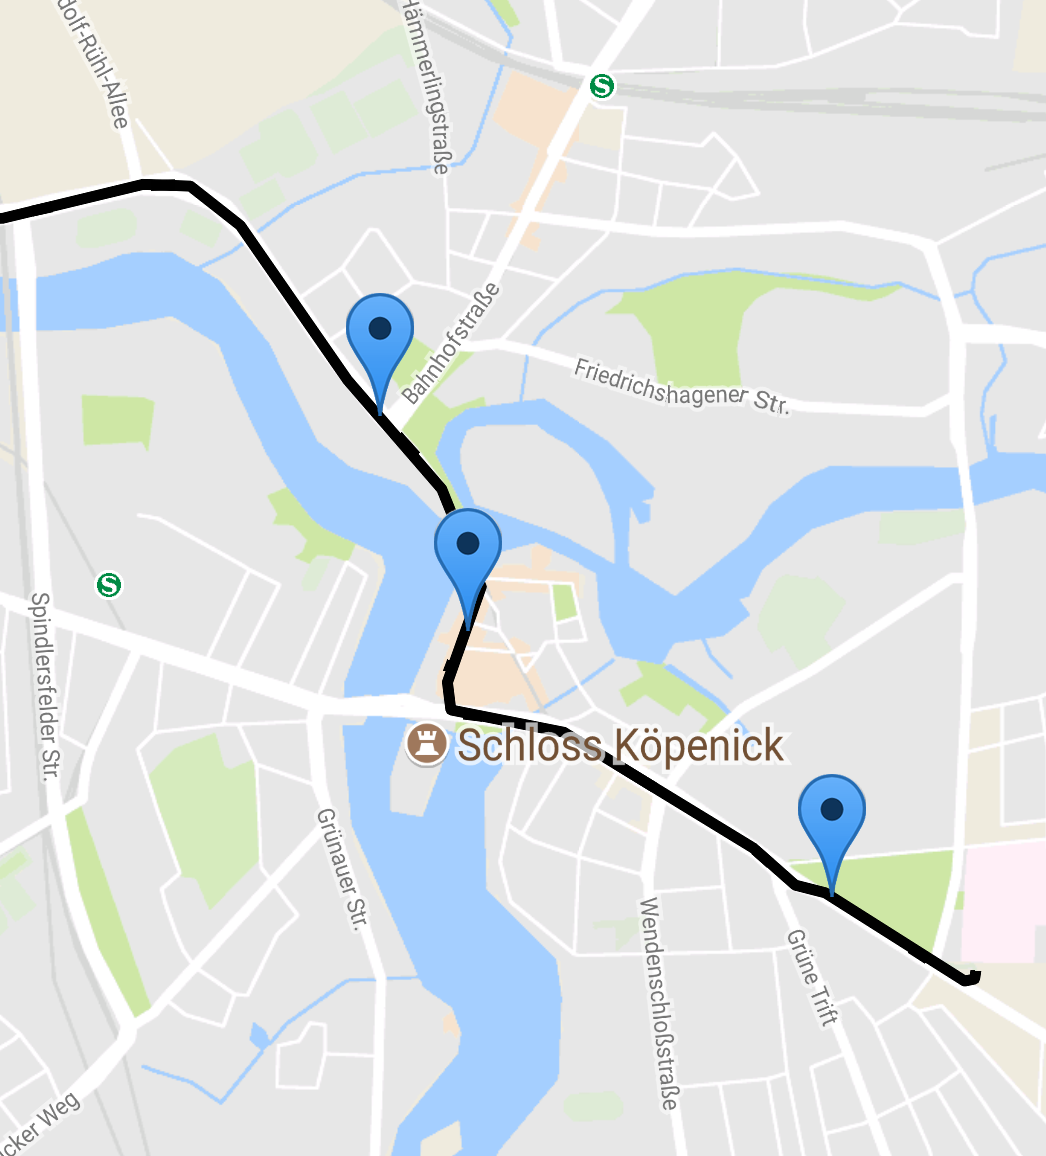
\includegraphics[width=8cm]{res/Route.png}
	\caption{Beispiel f�r Route mit 3 Fahrzeugen}
	\label{img:route}
\end{figure}

\section{Deployment / Runtime}